%------------------------------------------------
%
% Flow.tex 
%
% This section introduces the incident management
% process flow.
%------------------------------------------------
\section[Attività di processo]{attività di processo}
\label{im-flow}
Nella seguente sezione viene riportato il flusso delle attività presenti nel processo che gli operatori del \english{Service Desk} devono seguire in caso di incidente. In Figura \ref{im-flow-img} è visualizzato un diagramma di flusso rappresentante le attività, mentre ogni singolo \english{step} è elencato in Tabella \ref{im-flow-table}, mentre in Figura \ref{im-flow-life-cycle-img} è visualizzato il ciclo di vita di un \english{ticket}.

\begin{figure}[htbp]
\centering
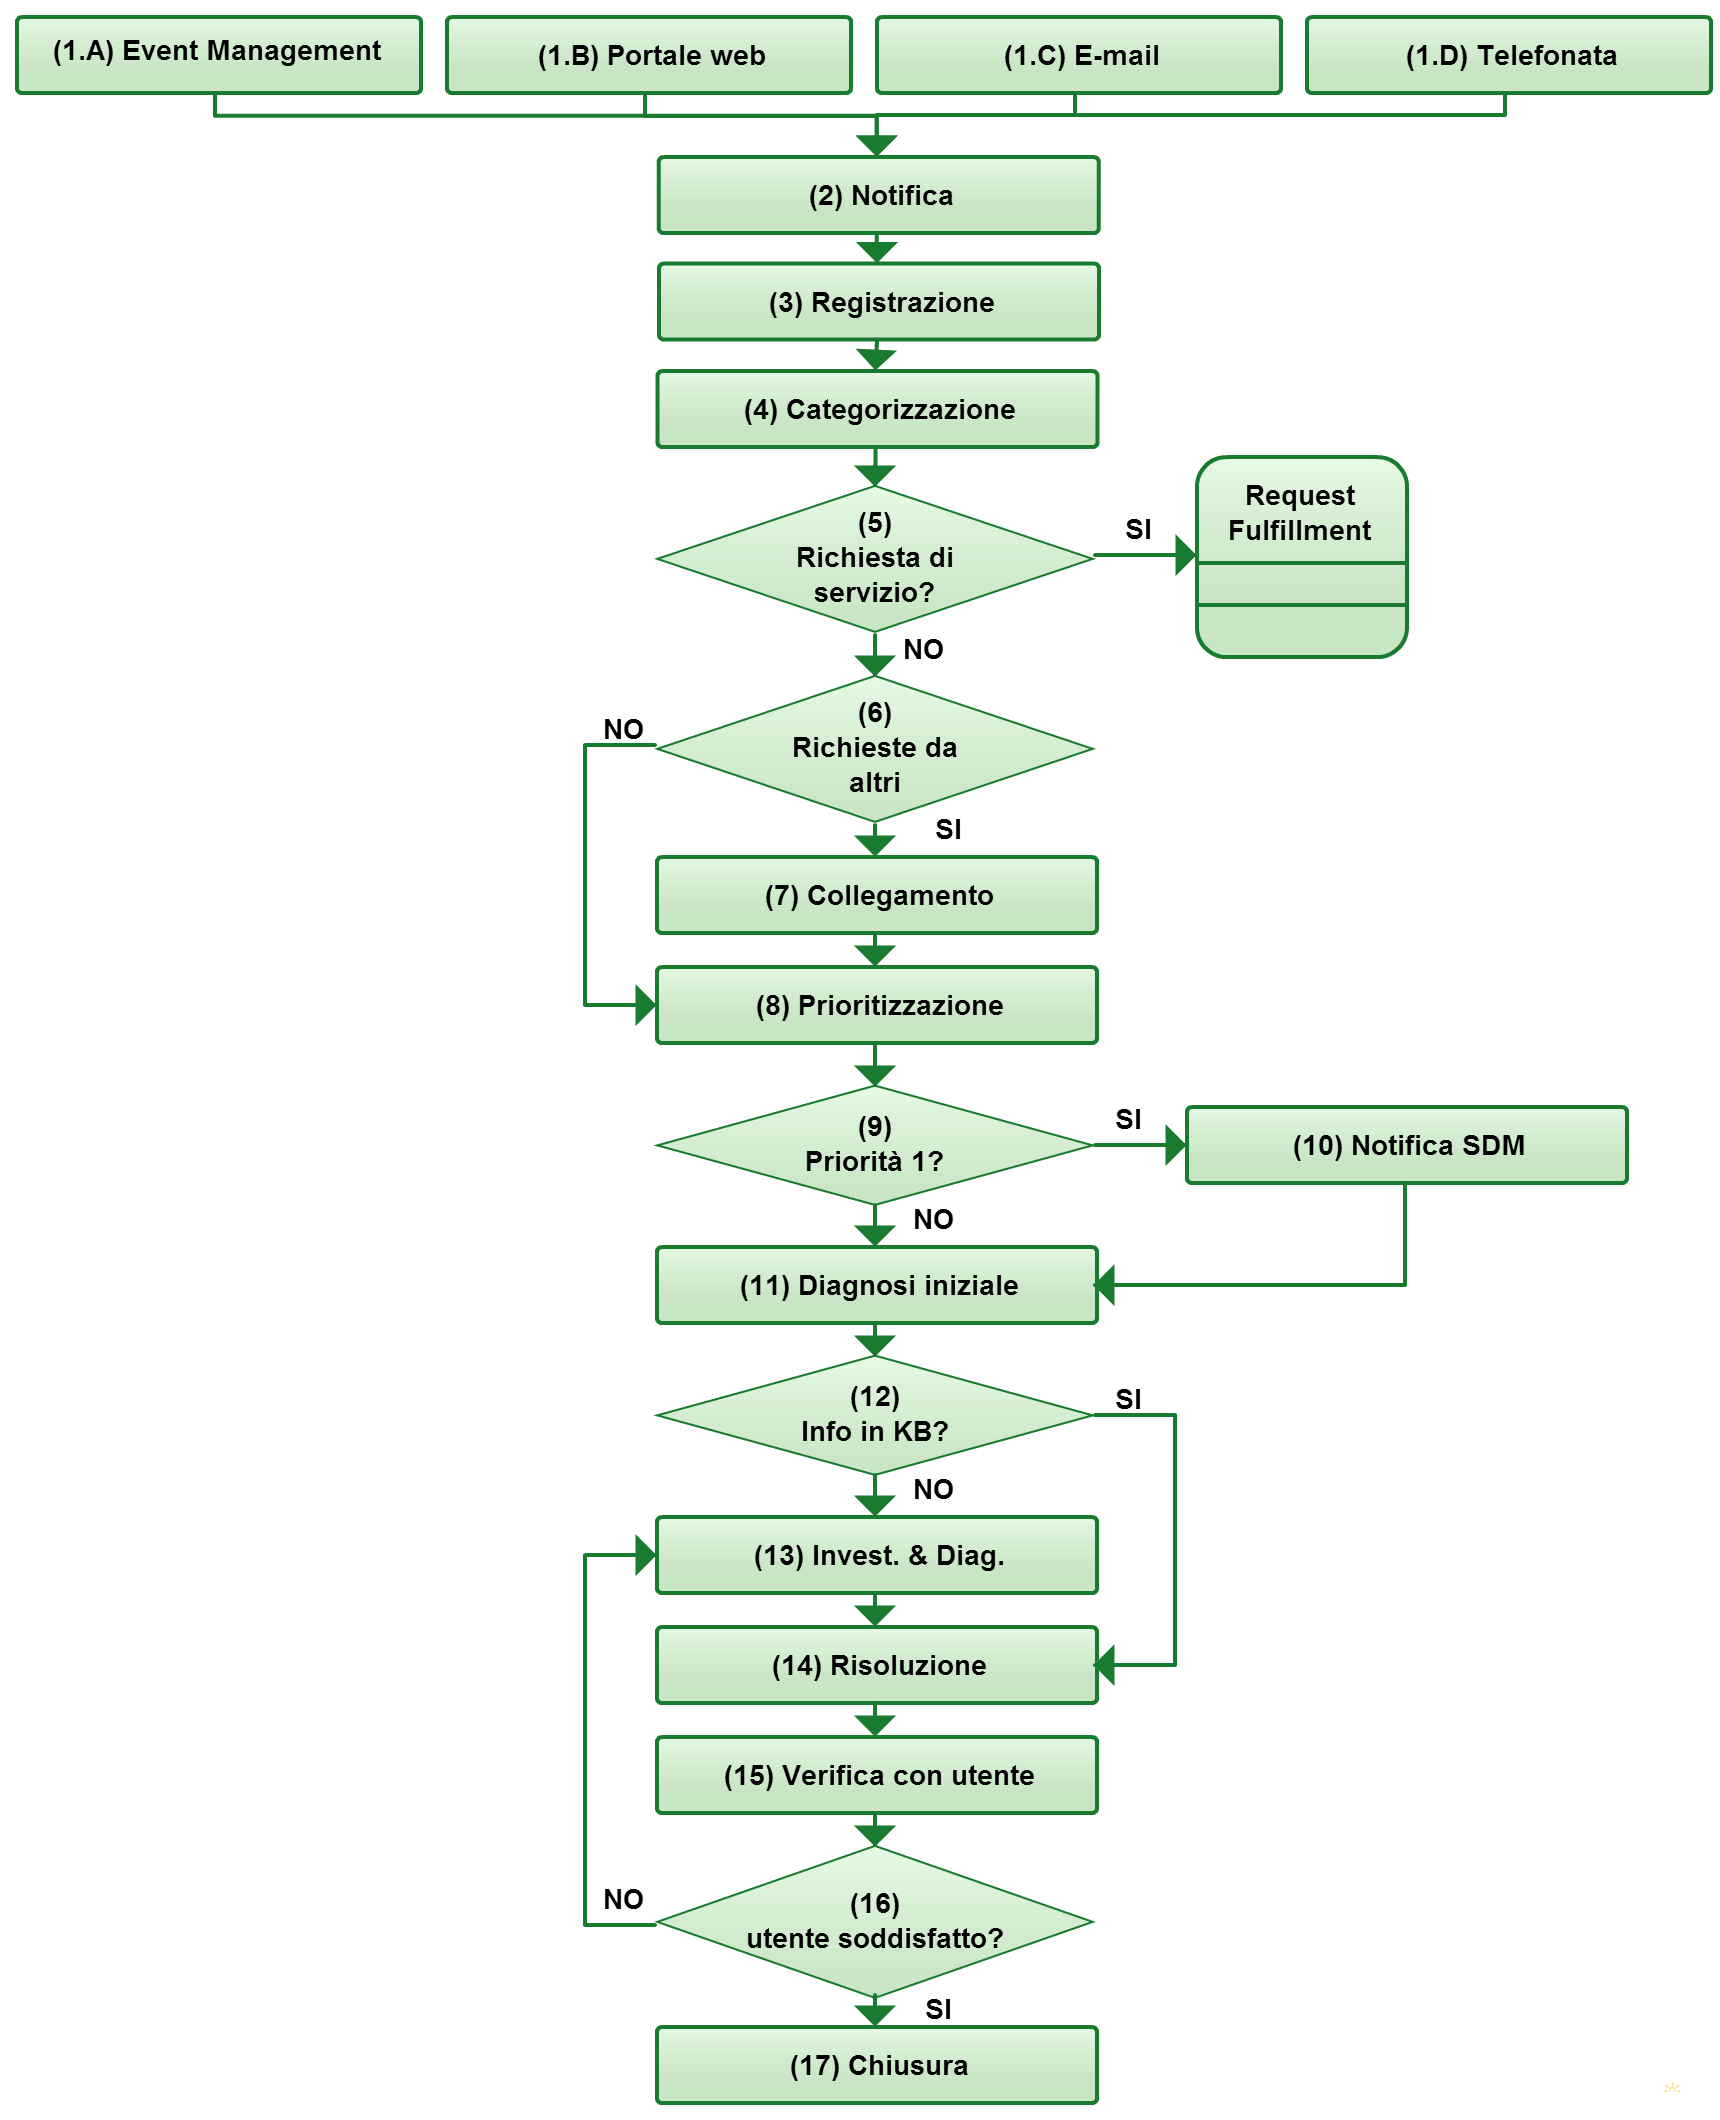
\includegraphics[scale=0.3]{Images/Diagrams/Incident_Management.png}
\caption{Flusso attività del processo di \ac{Incident-Management}}
\label{im-flow-img}
\end{figure}

\begin{center}
\begin{longtable}{| p{3cm} | p{2cm} | p {7cm} |}
\caption{Elenco attività di processo}
\label{im-flow-table}\\
\hline
\multicolumn{1}{| c |}{\textbf{Ruolo}} & \multicolumn{1}{| c |}{\textbf{Step}} & \multicolumn{1}{| c |}{\textbf{Descrizione}}\\
\hline
\endfirsthead
\hline
\multicolumn{1}{| c |}{\textbf{Ruolo}} & \multicolumn{1}{| c |}{\textbf{Step}} & \multicolumn{1}{| c |}{\textbf{Descrizione}}\\
\hline
\endhead
Utente & 1 & Gli incidenti possono essere riportati dagli utenti o dallo staff tecnico attraverso diversi canali di comunicazione (vedi Sezione \ref{sd-contact-mode}). Gli incidenti possono anche essere riportati attraverso l'uso di \english{tool} automatici a supporto del processo di \ac{Event-Management}.\\
\hline
\multirow{16}{*}{Staff tecnico} & 2 & Le successive attività non possono avvenire fino a che non viene notificato un incidente (tramite \english{ticket}) allo staff tecnico del \english{Service Desk}. E' necessario che lo staff tecnico presti attenzione a tutti gli strumenti che possono notificare un \english{ticket}.\\
\cline{2-3}
& 3 & Tutti gli incidenti devono essere registrati, con aggiunta di data/ora di quando l'incidente è stato notificato al \english{Service Desk} attraverso i diversi canali di comunicazione (vedi Sezione \ref{sd-contact-mode}). Tutte le informazioni rilevanti alla natura dell'incidente devono essere registrate, affinché gruppi di supporto avanzati possano entrare a conoscenza di tutti i dettagli tecnici.\\
\cline{2-3}
& 4 & Tutti gli incidenti sono relativi ad uno dei servizi esposti nel \english{Service Catalogue}. Qualora un utente riportasse una richiesta che non si riferisce a nessuno dei servizi esposti nel \english{Service Catalogue} allora tale richiesta non rappresenta un incidente.\\
\cline{2-3}
& 5 & Se si è in presenza di una richiesta di servizio mascherata come incidente allora essa deve essere reindirizzata al processo di \ac{Request-Fulfillment} che la tratterà nel modo più opportuno.\\
\cline{2-3}
& 6 & Si è in presenza di un incidente riportato da diversi utenti?\\
\cline{2-3}
& 7 & Se altri utenti hanno riportato la stessa richiesta, essa sarà collegata alle altre già riportate. Il fatto che più persone riportino la stessa richiesta significa che l'impatto dell'incidente è più ampio di quanto riportato inizialmente. L'impatto deve essere registrato sulla base delle attuali conoscenze.\\
\cline{2-3}
& 8 & Prima che la priorità di un incidente sia impostata è necessario stabilire la sua gravità ed il suo impatto, successivamente si utilizzerà la Tabella \ref{im-management-priority-table} per determinarne la priorità.\\
\cline{2-3}
& 9 & Si tratta di un incidente grave? (incidente a priorità 1).\\
\cline{2-3}
& 10 & Se siamo in presenza di un incidente grave significa che il servizio non è disponibile oppure non lo è in maggior parte. E' necessario notificare coloro che rivestano i seguenti ruoli \english{Service-Desk-Supervisior} e \english{Service-Desk-Manager}.\\
\cline{2-3}
& 11 & Se l'incidente è stato indirizzato presso il \english{Service Desk}, allora il \english{Service Desk Analyst} deve avviare la diagnosi iniziale usando \english{script} di diagnostica ed informazioni sui \english{Known Errors} al fine di scovare tutti i sintomi dell'incidente e determinare esattamente cosa non ha funzionato. L'\english{analyst} utilizzerà le informazioni raccolte per iniziare una ricerca nella \ac{Knowledge-Base} al fine di trovare la soluzione appropriata. Se possibile esso risolverà e chiuderà l'incidente se la risoluzione ha avuto successo.\\
\cline{2-3}
& 12 & Verificare se le informazioni presenti nella \ac{Knowledge-Base} sono sufficienti a risolvere l'incidente.\\
\cline{2-3}
& 13 & Se le informazioni presenti nella \ac{Knowledge-Base} non fossero sufficienti a risolvere l'incidente allora è necessario assegnarne la gestione al gruppo che supporta il servizio, che ricercherà le cause e opzioni di rimedio.\\
\cline{2-3}
& 14 & Dopo che una possibile soluzione è stata determinata, o attraverso la \english{Knolwledge-Base} oppure attraverso ricerca, si applica la soluzione che dovrebbe risolvere il problema.\\
\cline{2-3}
& 15 & Verifica con l'utente che la risoluzione lo abbia rimesso nelle condizioni di poter riprendere le sue mansioni. La risoluzione di un incidente non richiede che le cause sottostanti siano corrette, perché l'importante in questa fase non è curare le cause ma correggere i sintomi.\\
\cline{2-3}
& 16 & Se l'utente è soddisfatto della risoluzione allora si può procedere con la chiusura altrimenti si continuerà con l'investigazione a la diagnosi.\\
\cline{2-3}
& 17 & Il \english{Service Desk} deve controllare che l'incidente sia completamente risolto e che l'utente sia soddisfatto ed abbia acconsentito alla sua chiusura. Il \english{Service Desk} deve controllare anche le seguenti:
\begin{itemize}
\item{\textbf{categorizzazione della chiusura}: controllare e confermare che la categorizzazione iniziale fosse corretta o qualora fosse rilevata errata, aggiornare il \english{record} in modo da memorizzare una corretta categorizzazione.}
\item{\textbf{soddisfazione utente}: redigere un sommario sulla soddisfazione percepita dall'utente.}
\item{\textbf{documentazione}: rintracciare eventuali dettagli e assicurare che \english{incident record} sia documentato appieno cosicché sia presente uno storico con sufficiente livello di dettaglio.}
\item{\textbf{problema continuo o ricorrente}: Determinare se è possibile che l'incidente possa ripetersi e decidere quali azioni preventive sono necessarie per evitarlo. In collaborazione con il processo di \ac{Problem-Management} inoltrare un \english{record} in tutti quei casi in cui un'azione preventiva sia avviata.}
\item{\textbf{chiusura formale}: chiusura formale dell'\english{incident-record}.}
\end{itemize}\\
\hline
\end{longtable}
\end{center}

\begin{figure}[htbp]
\centering
\includegraphics[scale=0.25]{Images/Diagrams/Ticket_life_cycle.png}
\caption{Ciclo di vita di un \english{ticket}}
\label{im-flow-life-cycle-img}
\end{figure}